\documentclass[11pt,a4paper]{article}

%% ── Core packages ──────────────────────────────────────────────────────────
\usepackage[T1]{fontenc}
\usepackage[utf8]{inputenc}
\usepackage[top=22mm,bottom=22mm,left=20mm,right=20mm]{geometry}
\usepackage{microtype}
\usepackage{lmodern}

%% ── Colour ─────────────────────────────────────────────────────────────────
\usepackage[table]{xcolor}
\definecolor{PedBlue}{HTML}{1B4F8A}
\definecolor{PedTeal}{HTML}{2A8C8C}
\definecolor{PedGold}{HTML}{C9962C}
\definecolor{PedLight}{HTML}{EBF3FB}
\definecolor{PedRule}{HTML}{B8D4F0}
\definecolor{TableHead}{HTML}{D6E8F7}
\definecolor{TableAlt}{HTML}{F4F9FE}
\definecolor{WarnAmber}{HTML}{FFF3CD}
\definecolor{WarnBorder}{HTML}{C9962C}
\definecolor{GrayText}{HTML}{5A6070}
\definecolor{SpecimenGray}{HTML}{CCCCCC}

%% ── Typography ─────────────────────────────────────────────────────────────
\usepackage{helvet}
\renewcommand{\familydefault}{\sfdefault}

%% ── Layout & tables ────────────────────────────────────────────────────────
\usepackage{array}
\usepackage{booktabs}
\usepackage{colortbl}
\usepackage{tabularx}
\usepackage{multirow}
\usepackage{multicol}
\usepackage{enumitem}
\usepackage{parskip}
\usepackage{setspace}
\usepackage{ragged2e}

%% ── Graphics ───────────────────────────────────────────────────────────────
\usepackage{graphicx}
\usepackage{tikz}
\usetikzlibrary{positioning,calc,shapes.geometric,backgrounds,patterns,decorations.pathmorphing}
\usepackage[most]{tcolorbox}
\usepackage{fontawesome5}

%% ── Watermark ──────────────────────────────────────────────────────────────
\usepackage{eso-pic}
\usepackage{amsmath}
\usepackage{amssymb}

%% ── Links ──────────────────────────────────────────────────────────────────
\usepackage[hidelinks]{hyperref}

%% ────────────────────────────────────────────────────────────────────────────
%% SPECIMEN watermark (every page)
%% ────────────────────────────────────────────────────────────────────────────
\AddToShipoutPictureBG{%
  \begin{tikzpicture}[remember picture,overlay]
    \node[rotate=45, opacity=0.10,
          font=\fontsize{72}{72}\selectfont\bfseries,
          text=SpecimenGray]
      at (current page.center) {SPECIMEN};
  \end{tikzpicture}%
}

%% ────────────────────────────────────────────────────────────────────────────
%% tcolorbox styles
%% ────────────────────────────────────────────────────────────────────────────
\tcbuselibrary{skins,breakable}

\tcbset{
  pednote/.style={
    enhanced,
    breakable,
    colback=white,
    colframe=PedBlue,
    colbacktitle=PedBlue,
    coltitle=white,
    fonttitle=\bfseries\small,
    arc=3pt,
    boxrule=0.8pt,
    top=6pt, bottom=6pt, left=8pt, right=8pt,
    titlerule=0pt,
    attach boxed title to top left={yshift=-2pt, xshift=8pt},
    boxed title style={arc=2pt, boxrule=0pt, colback=PedBlue}
  },
  pedteal/.style={
    enhanced,
    breakable,
    colback=white,
    colframe=PedTeal,
    colbacktitle=PedTeal,
    coltitle=white,
    fonttitle=\bfseries\small,
    arc=3pt,
    boxrule=0.8pt,
    top=6pt, bottom=6pt, left=8pt, right=8pt,
    titlerule=0pt,
    attach boxed title to top left={yshift=-2pt, xshift=8pt},
    boxed title style={arc=2pt, boxrule=0pt, colback=PedTeal}
  },
  pedinfostrip/.style={
    enhanced,
    colback=PedLight,
    colframe=PedRule,
    arc=3pt,
    boxrule=0.6pt,
    top=5pt, bottom=5pt, left=10pt, right=10pt
  },
  pedwarn/.style={
    enhanced,
    colback=WarnAmber,
    colframe=WarnBorder,
    arc=3pt,
    boxrule=0.8pt,
    top=5pt, bottom=5pt, left=8pt, right=8pt
  },
  pedgold/.style={
    enhanced,
    colback=white,
    colframe=PedGold,
    colbacktitle=PedGold,
    coltitle=white,
    fonttitle=\bfseries\small,
    arc=3pt,
    boxrule=0.8pt,
    top=6pt, bottom=6pt, left=8pt, right=8pt,
    titlerule=0pt,
    attach boxed title to top left={yshift=-2pt, xshift=8pt},
    boxed title style={arc=2pt, boxrule=0pt, colback=PedGold}
  }
}

%% ────────────────────────────────────────────────────────────────────────────
%% Custom commands
%% ────────────────────────────────────────────────────────────────────────────
\newcommand{\sectionrule}[1]{%
  \vspace{2pt}%
  {\color{PedBlue}\rule{\linewidth}{1.5pt}}\\[-4pt]%
  {\color{PedTeal}\rule{\linewidth}{0.4pt}}%
  \vspace{2pt}%
}

\newcommand{\fieldlabel}[1]{{\footnotesize\color{GrayText}\textbf{#1}}}
\newcommand{\fieldval}[1]{{\small #1}}
\newcommand{\highlight}[1]{{\color{PedBlue}\textbf{#1}}}
\newcommand{\tealtext}[1]{{\color{PedTeal}\textbf{#1}}}
\newcommand{\goldtext}[1]{{\color{PedGold}\textbf{#1}}}

\setlength{\parskip}{4pt}
\setlength{\parindent}{0pt}

%% ════════════════════════════════════════════════════════════════════════════
\begin{document}
\pagestyle{plain}

%% ────────────────────────────────────────────────────────────────────────────
%% HEADER
%% ────────────────────────────────────────────────────────────────────────────
\begin{tikzpicture}[remember picture, overlay]
  \fill[PedBlue] (current page.north west)
    rectangle +(\paperwidth, -28mm);
  \fill[PedTeal] (current page.north west) ++(0,-28mm)
    rectangle +(\paperwidth, -4mm);
\end{tikzpicture}

\vspace*{-6mm}
\begin{minipage}[t]{0.62\linewidth}
  \vspace{0pt}
  {\color{white}\fontsize{20}{24}\selectfont\textbf{Meridian Children's Hospital}}\\[1mm]
  {\color{PedRule}\small Department of Pediatric Medicine \& Subspecialty Services}\\[1mm]
  {\color{white!80!PedBlue}\footnotesize
    47 Lakeview Boulevard, Suite 300 \quad|\quad Harborfield, ON M4K 2R7\\
    Tel: (416) 555-0182 \quad|\quad Fax: (416) 555-0199 \quad|\quad
    \href{mailto:consults@meridianchildrens.ca}{consults@meridianchildrens.ca}
  }
\end{minipage}%
\hfill
\begin{minipage}[t]{0.34\linewidth}
  \vspace{0pt}
  \raggedleft
  \begin{tikzpicture}
    \fill[white,opacity=0.12] (0,0) circle (1.1cm);
    \draw[white, line width=1.5pt] (0,0) circle (1.0cm);
    \node[white, font=\fontsize{28}{28}\selectfont] at (0,0.05) {\faChild};
    \node[white, font=\fontsize{7}{7}\selectfont\bfseries] at (0,-0.72) {PEDIATRICS};
  \end{tikzpicture}
\end{minipage}

\vspace{14mm}

%% ── Document title bar ──────────────────────────────────────────────────────
\begin{tcolorbox}[
  enhanced,
  colback=PedLight,
  colframe=PedBlue,
  arc=4pt,
  boxrule=1pt,
  top=7pt, bottom=7pt, left=12pt, right=12pt
]
  \begin{minipage}{0.65\linewidth}
    {\fontsize{15}{18}\selectfont\color{PedBlue}\textbf{PEDIATRIC CLINICAL CONSULTATION NOTE}}\\[1pt]
    {\small\color{GrayText} Subspecialty: \tealtext{Pediatric Endocrinology \& Metabolism}}
  \end{minipage}%
  \hfill
  \begin{minipage}{0.32\linewidth}
    \raggedleft
    {\footnotesize\color{GrayText}
      \faCalendar\; \textbf{Date:} July 22, 2025\\[2pt]
      \faFile\; \textbf{Note \#:} MCH-2025-00847\\[2pt]
      \faHospital\; \textbf{Service:} Outpatient Consult
    }
  \end{minipage}
\end{tcolorbox}

\vspace{4mm}

%% ────────────────────────────────────────────────────────────────────────────
%% PATIENT DEMOGRAPHICS
%% ────────────────────────────────────────────────────────────────────────────
\begin{tcolorbox}[pednote, title={\faUser\enspace Patient Demographics}]
  \begin{tabularx}{\linewidth}{@{} l X l X @{}}
    \fieldlabel{Patient Name}  & \fieldval{Oliver James Hargrove} &
    \fieldlabel{Date of Birth} & \fieldval{March 4, 2016 (Age: 9 yrs 4 mo)} \\[4pt]
    \fieldlabel{MRN}           & \fieldval{MCH-096-2241} &
    \fieldlabel{Health Card}   & \fieldval{4782-643-210 (ON)} \\[4pt]
    \fieldlabel{Sex}           & \fieldval{Male} &
    \fieldlabel{Preferred Name}& \fieldval{Ollie} \\[4pt]
    \fieldlabel{Address}       & \multicolumn{3}{l}{\fieldval{22 Birchwood Crescent, Harborfield, ON M5P 1T9}} \\[4pt]
    \fieldlabel{Guardian}      & \fieldval{Margaret \& Daniel Hargrove (Parents)} &
    \fieldlabel{Phone}         & \fieldval{(416) 555-0243} \\[4pt]
    \fieldlabel{Language}      & \fieldval{English (primary)} &
    \fieldlabel{Interpreter}   & \fieldval{Not required} \\
  \end{tabularx}
\end{tcolorbox}

\vspace{3mm}

%% ── Referring / Consulting physicians (two minipages) ───────────────────────
\begin{minipage}[t]{0.48\linewidth}
\begin{tcolorbox}[pedinfostrip, top=7pt, bottom=7pt]
  {\small\color{PedBlue}\textbf{\faUserMd\enspace Referring Physician}}\\[4pt]
  \fieldlabel{Name}\quad \fieldval{Dr. Sandra Wolfe, MD, CCFP}\\[2pt]
  \fieldlabel{Clinic}\quad \fieldval{Northgate Family Health Team}\\[2pt]
  \fieldlabel{Phone}\quad \fieldval{(416) 555-0371}\\[2pt]
  \fieldlabel{Fax}\quad \fieldval{(416) 555-0372}\\[2pt]
  \fieldlabel{Referral Date}\quad \fieldval{June 30, 2025}\\[2pt]
  \fieldlabel{Priority}\quad {\color{PedGold}\textbf{Routine — 3 weeks}}
\end{tcolorbox}
\end{minipage}\par
%
\begin{minipage}[t]{0.48\linewidth}
\hfill
\begin{tcolorbox}[pedinfostrip, top=7pt, bottom=7pt]
  {\small\color{PedTeal}\textbf{\faStethoscope\enspace Consulting Physician}}\\[4pt]
  \fieldlabel{Name}\quad \fieldval{Dr. Priya Mehta, MD, FRCPC}\\[2pt]
  \fieldlabel{Specialty}\quad \fieldval{Pediatric Endocrinology}\\[2pt]
  \fieldlabel{Phone}\quad \fieldval{(416) 555-0182 x204}\\[2pt]
  \fieldlabel{Pager}\quad \fieldval{MCH-P-2047}\\[2pt]
  \fieldlabel{Fellow}\quad \fieldval{Dr. Lucas Chen, MD (PGY-5)}\\[2pt]
  \fieldlabel{Location}\quad \fieldval{MCH Clinic 3, Level 2}
\end{tcolorbox}
\end{minipage}

\vspace{4mm}

%% ────────────────────────────────────────────────────────────────────────────
%% REASON FOR CONSULTATION
%% ────────────────────────────────────────────────────────────────────────────
\begin{tcolorbox}[pednote, title={\faSearch\enspace Reason for Consultation}]
  Referral for evaluation of \highlight{short stature and growth deceleration} in a 9-year-old
  male. Parents report Ollie has been consistently below the 3rd percentile for height over
  the past 18 months and is significantly shorter than his classmates. Growth velocity has
  been estimated at approximately \textbf{3.8 cm/year} over the preceding 12 months, which
  is below the expected 5--6 cm/year for his age. No pubertal changes noted. Referral also
  includes concern regarding mild \highlight{thyroid function abnormalities} on routine
  screening bloodwork (TSH mildly elevated at 5.2 mIU/L, free T4 low-normal).
\end{tcolorbox}

\vspace{3mm}

%% ────────────────────────────────────────────────────────────────────────────
%% HISTORY OF PRESENTING ILLNESS
%% ────────────────────────────────────────────────────────────────────────────
\begin{tcolorbox}[pednote, title={\faClipboardList\enspace History of Presenting Illness}]

\textbf{\color{PedTeal}Growth History:}
Ollie was born at 38 weeks gestation via spontaneous vaginal delivery.
Birth weight: 3.02 kg (25th percentile). Birth length: 49 cm (25th percentile).
Head circumference: 34.5 cm (50th percentile). NICU stay was not required.
He tracked along the 25th percentile through infancy. A progressive decline in
growth velocity was first documented at age 7 (April 2023), at which time he
crossed below the 10th percentile. By his 8-year annual check-up (March 2024),
he had fallen below the 3rd percentile for height.

\medskip
\textbf{\color{PedTeal}Associated Symptoms:}
\begin{itemize}[leftmargin=1.4em, itemsep=2pt, topsep=2pt]
  \item Mild fatigue, particularly noted in afternoons; parents initially
        attributed this to a demanding school schedule.
  \item Increased sensitivity to cold temperatures over the past 6 months.
  \item Mild constipation (bowel movements every 2--3 days); no blood per rectum.
  \item Slight puffiness noted around the eyes in the mornings (reported by mother).
  \item Appetite described as ``picky but adequate''; no dysphagia, no vomiting.
  \item No polyuria, polydipsia, or headaches.
  \item No visual changes or neurological symptoms.
\end{itemize}

\medskip
\textbf{\color{PedTeal}Pubertal Development:}
No breast/testicular enlargement. No axillary or pubic hair. No acne.
Tanner Stage I assessment confirmed. Parents confirm no early pubertal signs
at home. Family history of constitutional delay: father reports onset of
puberty at approximately age 15.

\end{tcolorbox}

\vspace{3mm}

%% ────────────────────────────────────────────────────────────────────────────
%% PAST MEDICAL / SURGICAL / MEDICATIONS
%% ────────────────────────────────────────────────────────────────────────────
\begin{minipage}[t]{0.48\linewidth}
\begin{tcolorbox}[pedteal,
  title={\faNotesMedical\enspace Past Medical History},
  height=62mm]
  \begin{itemize}[leftmargin=1.2em, itemsep=3pt, topsep=0pt, label={\color{PedTeal}\textbullet}]
    \item Recurrent otitis media (ages 3--5); bilateral PE tubes
          inserted April 2020; extruded spontaneously 2021.
    \item Mild allergic rhinitis; managed with cetirizine PRN.
    \item Iron-deficiency anemia at age 5; resolved with supplementation.
    \item No prior hospitalizations beyond birth admission.
    \item No chronic illness previously documented.
    \item Immunizations up to date per provincial schedule.
  \end{itemize}
\end{tcolorbox}
\end{minipage}\par
%
\begin{minipage}[t]{0.48\linewidth}
\hfill
\begin{tcolorbox}[pedteal,
  title={\faPills\enspace Medications \& Allergies},
  height=62mm]
  \textbf{\color{PedTeal}Current Medications:}
  \begin{itemize}[leftmargin=1.2em, itemsep=2pt, topsep=2pt, label={\color{PedTeal}\textbullet}]
    \item Cetirizine 5 mg PO once daily PRN (rhinitis)
    \item Vitamin D$_3$ 400 IU PO once daily
    \item Multivitamin (pediatric formulation) once daily
  \end{itemize}
  \medskip
  \textbf{\color{PedTeal}Allergies / Intolerances:}
  \begin{itemize}[leftmargin=1.2em, itemsep=2pt, topsep=2pt, label={\color{WarnBorder}\faExclamationTriangle}]
    \item Penicillin --- urticaria (age 4)
    \item No food allergies documented
  \end{itemize}
\end{tcolorbox}
\end{minipage}

\vspace{3mm}

%% ────────────────────────────────────────────────────────────────────────────
%% FAMILY / SOCIAL HISTORY
%% ────────────────────────────────────────────────────────────────────────────
\begin{minipage}[t]{0.48\linewidth}
\begin{tcolorbox}[pednote,
  title={\faUsers\enspace Family History},
  height=55mm]
  \begin{itemize}[leftmargin=1.2em, itemsep=3pt, topsep=0pt, label={\color{PedBlue}\textbullet}]
    \item Father (Daniel, 42): \textbf{Constitutional delay of growth and puberty}
          (CDGP); final adult height 170 cm.
    \item Mother (Margaret, 40): Hashimoto's thyroiditis, on levothyroxine.
    \item Maternal grandmother: Type 2 diabetes mellitus.
    \item Paternal uncle: Celiac disease.
    \item No family history of Turner syndrome, growth hormone deficiency,
          or pituitary tumours.
    \item No consanguinity.
  \end{itemize}
\end{tcolorbox}
\end{minipage}\par
%
\begin{minipage}[t]{0.48\linewidth}
\hfill
\begin{tcolorbox}[pednote,
  title={\faHome\enspace Social History},
  height=55mm]
  \begin{itemize}[leftmargin=1.2em, itemsep=3pt, topsep=0pt, label={\color{PedBlue}\textbullet}]
    \item Lives with both parents and one younger sibling (age 6, F, healthy).
    \item Father works as a civil engineer; mother is a registered nurse.
    \item Attends Grade 4 at Maplewood Public School; above-average academic performance.
    \item Active in soccer and swimming.
    \item Diet: generally balanced; consumes dairy; no gluten restriction.
    \item No tobacco, alcohol, or substance exposure in the home.
    \item No recent international travel.
  \end{itemize}
\end{tcolorbox}
\end{minipage}

\vspace{4mm}

%% ────────────────────────────────────────────────────────────────────────────
%% PHYSICAL EXAMINATION
%% ────────────────────────────────────────────────────────────────────────────
\begin{tcolorbox}[pedgold, title={\faHeartbeat\enspace Physical Examination}]

\begin{minipage}[t]{0.50\linewidth}
  \vspace{0pt}
  \textbf{\color{PedGold}Vital Signs \& Anthropometrics}\\[4pt]
  \begin{tabular}{@{} l l l @{}}
    \toprule
    \rowcolor{TableHead}
    \textbf{Parameter} & \textbf{Value} & \textbf{Percentile} \\
    \midrule
    Height             & 119.4 cm       & $<$3rd (WHO)        \\
    Weight             & 21.6 kg        & 5th                 \\
    BMI                & 15.2 kg/m$^2$  & 18th                \\
    Head Circ.         & 51.8 cm        & 50th                \\
    BP                 & 95/62 mmHg     & Normal              \\
    HR                 & 74 bpm         & Normal              \\
    RR                 & 18 bpm         & Normal              \\
    SpO$_2$            & 99\%           & ---                 \\
    Temperature        & 36.8\textdegree C & Afebrile         \\
    \bottomrule
  \end{tabular}

  \medskip
  \fieldlabel{Bone Age (left hand X-ray):}\\
  \fieldval{Estimated \textbf{7.5 years} (chronological age 9.4 yrs)}\\[2pt]
  \fieldlabel{Predicted Adult Height (Bayley-Pinneau):}\\
  \fieldval{\textbf{167 cm} (5th--10th percentile)}\\[2pt]
  \fieldlabel{Mid-Parental Height:}\\
  \fieldval{\textbf{171.5 cm} [Father 170 cm, Mother 164 cm]}
\end{minipage}%
\hfill
\begin{minipage}[t]{0.46\linewidth}
  \vspace{0pt}
  \textbf{\color{PedGold}Systemic Examination}\\[4pt]
  {\small
  \textit{General:} Well-nourished, alert, cooperative boy. No acute distress.
  Dysmorphic features absent. Proportionate short stature.\medskip

  \textit{HEENT:} Normocephalic. Mild periorbital puffiness bilaterally.
  Thyroid gland mildly enlarged, non-tender, smooth texture, no nodules palpable.
  No cervical lymphadenopathy.\medskip

  \textit{Skin:} Mildly cool, dry skin texture. No jaundice, no pallor.
  No striae, no acanthosis. Normal hair texture.\medskip

  \textit{Cardiovascular:} Regular rate and rhythm. No murmurs.
  Peripheral pulses 2+ bilaterally.\medskip

  \textit{Respiratory:} Clear to auscultation bilaterally.\medskip

  \textit{Abdomen:} Soft, non-tender. No organomegaly.
  No abdominal masses.\medskip

  \textit{Neurological:} Cranial nerves II--XII intact.
  Deep tendon reflexes 2+ and symmetric. Normal gait.\medskip

  \textit{Pubertal Assessment:} Tanner Stage I (genitalia, pubic hair).
  Testicular volume 2 mL bilaterally (Prader orchidometer).
  }
\end{minipage}

\end{tcolorbox}

\vspace{4mm}

%% ────────────────────────────────────────────────────────────────────────────
%% GROWTH CURVE TABLE
%% ────────────────────────────────────────────────────────────────────────────
\begin{tcolorbox}[pedteal, title={\faChartLine\enspace Longitudinal Growth Record (WHO/CDC Reference)}]

\renewcommand{\arraystretch}{1.28}
\begin{tabularx}{\linewidth}{@{} l l >{\centering\arraybackslash}X >{\centering\arraybackslash}X >{\centering\arraybackslash}X >{\centering\arraybackslash}X @{}}
  \toprule
  \rowcolor{TableHead}
  \textbf{Date} & \textbf{Age} & \textbf{Height (cm)} & \textbf{Ht \%ile} & \textbf{Weight (kg)} & \textbf{Wt \%ile} \\
  \midrule
  \rowcolor{white}
  Mar 2016 & Birth       & 49.0  & 25th       & 3.02  & 25th  \\
  \rowcolor{TableAlt}
  Sep 2016 & 6 mo        & 65.8  & 30th       & 7.48  & 35th  \\
  \rowcolor{white}
  Mar 2017 & 1 yr        & 74.6  & 28th       & 9.55  & 30th  \\
  \rowcolor{TableAlt}
  Mar 2018 & 2 yr        & 85.3  & 25th       & 12.10 & 28th  \\
  \rowcolor{white}
  Mar 2019 & 3 yr        & 93.4  & 22nd       & 14.20 & 22nd  \\
  \rowcolor{TableAlt}
  Mar 2020 & 4 yr        & 100.7 & 20th       & 15.90 & 20th  \\
  \rowcolor{white}
  Mar 2021 & 5 yr        & 107.4 & 18th       & 17.60 & 18th  \\
  \rowcolor{TableAlt}
  Mar 2022 & 6 yr        & 113.6 & 14th       & 18.90 & 15th  \\
  \rowcolor{white}
  Mar 2023 & 7 yr        & 118.2 & 8th        & 20.10 & 10th  \\
  \rowcolor{TableAlt}
  Mar 2024 & 8 yr        & \textbf{121.8} & \textbf{$<$3rd} & 20.90 & 7th \\
  \rowcolor{white}
  Jul 2025 & 9 yr 4 mo   & \highlight{119.4}$^*$ & \highlight{$<$3rd} & 21.60 & 5th \\
  \bottomrule
\end{tabularx}
\vspace{2pt}
{\footnotesize\color{GrayText}
$^*$ Today's measurement. Growth velocity: 3.8 cm/year (reference $\geq$5.0 cm/year for age).
Height standard deviation score (SDS): $-2.7$. Weight SDS: $-1.6$.}

\medskip
%% ── Inline growth bar chart ─────────────────────────────────────────────────
\textbf{\color{PedTeal}\small Height Velocity Trend (cm/year):}\\[4pt]
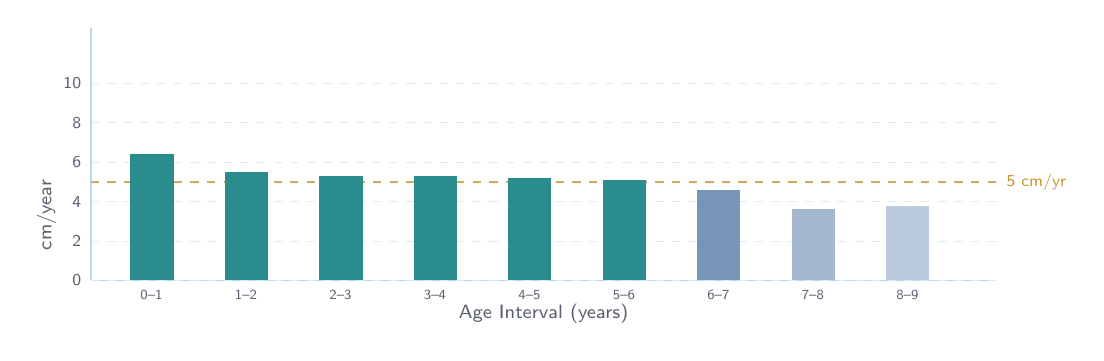
\begin{tikzpicture}[scale=1.0]
  % axis
  \draw[PedRule, line width=0.5pt] (0,0) -- (11.5,0);
  \draw[PedRule, line width=0.5pt] (0,0) -- (0,3.2);
  % grid lines
  \foreach \y/\label in {0/0,0.5/2,1.0/4,1.5/6,2.0/8,2.5/10}{
    \draw[PedRule!50, dashed, line width=0.3pt] (0,\y) -- (11.5,\y);
    \node[left, font=\fontsize{6}{6}\selectfont, text=GrayText] at (0,\y) {\label};
  }
  % reference line at 5 cm/yr
  \draw[PedGold!80, line width=0.8pt, dashed] (0,1.25) -- (11.5,1.25)
    node[right, font=\fontsize{6}{6}\selectfont, text=PedGold] {5 cm/yr};
  % bars: years 1,2,3,4,5,6,7 -> velocities in cm/yr
  % approximate velocities from table
  % 0-1yr: 25.6cm, 1-2yr:10.7, 2-3yr:8.1, 3-4yr:7.3, 4-5yr:6.7, 5-6yr:6.2,
  % 6-7yr:4.6, 7-8yr:3.6, 8-9yr(partial,14mo):~2.2 -> annualized 3.8
  \def\bw{0.55}
  \def\sc{0.25} % scale factor: 1cm/yr -> 0.25 units height
  % bar positions
  \foreach \x/\vel/\clr in {
    0.5/6.4/PedTeal,
    1.7/5.5/PedTeal,
    2.9/5.3/PedTeal,
    4.1/5.3/PedTeal,
    5.3/5.2/PedTeal,
    6.5/5.1/PedTeal,
    7.7/4.6/PedBlue!60,
    8.9/3.6/PedBlue!40,
    10.1/3.8/PedBlue!30}{
    \pgfmathsetmacro{\bh}{\vel*\sc}
    \fill[\clr] (\x,0) rectangle +(\bw,\bh);
  }
  % x labels
  \foreach \x/\lbl in {0.77/\text{0--1},1.97/\text{1--2},3.17/\text{2--3},
    4.37/\text{3--4},5.57/\text{4--5},6.77/\text{5--6},
    7.97/\text{6--7},9.17/\text{7--8},10.37/\text{8--9}}{
    \node[below, font=\fontsize{5.5}{5.5}\selectfont, text=GrayText]
      at (\x+\bw/2-0.275,0) {$\lbl$};
  }
  \node[below=5pt, font=\fontsize{7}{7}\selectfont, text=GrayText]
    at (5.75,0) {Age Interval (years)};
  \node[left=16pt, rotate=90, font=\fontsize{7}{7}\selectfont, text=GrayText]
    at (0,1.4) {cm/year};
\end{tikzpicture}

\end{tcolorbox}

\vspace{4mm}

%% ────────────────────────────────────────────────────────────────────────────
%% INVESTIGATIONS
%% ────────────────────────────────────────────────────────────────────────────
\begin{tcolorbox}[pednote, title={\faFlask\enspace Investigations}]

\begin{minipage}[t]{0.48\linewidth}
  \vspace{0pt}
  \textbf{\color{PedBlue}Bloodwork (Referring Physician --- June 28, 2025):}
  \renewcommand{\arraystretch}{1.2}
  \begin{tabular}{@{} l l l @{}}
    \toprule
    \rowcolor{TableHead}
    \textbf{Test} & \textbf{Result} & \textbf{Reference} \\
    \midrule
    TSH              & \textbf{5.2 mIU/L}\textsuperscript{\dag} & 0.5--4.5     \\
    Free T4          & 11.8 pmol/L       & 10.0--20.0   \\
    Free T3          & 4.1 pmol/L        & 3.5--7.8     \\
    TPO Ab           & \textbf{142 IU/mL}\textsuperscript{\dag} & $<$35        \\
    Anti-Tg Ab       & 68 IU/mL          & $<$40        \\
    CBC              & Normal            & ---          \\
    Ferritin         & 24 $\mu$g/L       & 15--150      \\
    CRP              & 1.2 mg/L          & $<$5         \\
    ESR              & 8 mm/hr           & $<$20        \\
    HbA1c            & 5.1\%             & $<$5.7\%     \\
    \bottomrule
  \end{tabular}
  {\footnotesize\color{WarnBorder}\dag\ Elevated / outside reference range.}
\end{minipage}%
\hfill
\begin{minipage}[t]{0.48\linewidth}
  \vspace{0pt}
  \textbf{\color{PedBlue}Additional Investigations (Today / Ordered):}
  \renewcommand{\arraystretch}{1.2}
  \begin{tabular}{@{} l l l @{}}
    \toprule
    \rowcolor{TableHead}
    \textbf{Test} & \textbf{Result} & \textbf{Status} \\
    \midrule
    IGF-1             & 78 ng/mL          & \textbf{Low}\textsuperscript{\dag}   \\
    IGFBP-3           & 2.1 mg/L          & Low-normal   \\
    GH stimulation    & ---               & Pending      \\
    LH / FSH          & Prepubertal       & Normal       \\
    Testosterone      & $<$0.3 nmol/L     & Prepubertal  \\
    Karyotype         & 46,XY             & Normal       \\
    Celiac panel      & Negative          & Normal       \\
    25-OH Vitamin D   & 38 nmol/L         & Insufficient \\
    Calcium / Phos    & Normal            & Normal       \\
    BMP               & Normal            & Normal       \\
    \bottomrule
  \end{tabular}
  {\footnotesize\color{WarnBorder}\dag\ IGF-1 SDS: $-2.1$ for age/sex.}

  \medskip
  \textbf{\color{PedBlue}Imaging:}\\[2pt]
  {\small
  \faXRay\ \textbf{Left hand/wrist X-ray} (July 22, 2025): Bone age 7.5 years
  (Greulich \& Pyle atlas). Delayed by approximately 1.9 years
  relative to chronological age.\\[3pt]
  \faMicroscope\ \textbf{Thyroid ultrasound} (ordered today): Pending.
  Will assess for echotexture changes consistent with autoimmune thyroiditis.
  }
\end{minipage}

\end{tcolorbox}

\vspace{4mm}

%% ────────────────────────────────────────────────────────────────────────────
%% ASSESSMENT
%% ────────────────────────────────────────────────────────────────────────────
\begin{tcolorbox}[pedgold, title={\faClipboardCheck\enspace Assessment \& Differential Diagnosis}]

\textbf{\color{PedGold}Primary Assessment:}\\[4pt]
A 9-year-4-month-old male presenting with progressive short stature (height SDS $-2.7$),
reduced growth velocity (3.8 cm/year), and bone age delay of 1.9 years in the
context of biochemical evidence of \highlight{Hashimoto's thyroiditis} with subclinical
hypothyroidism. The constellation of mildly elevated TSH, positive thyroid antibodies,
low-normal free T4, characteristic symptoms (fatigue, cold intolerance, constipation,
periorbital puffiness, dry skin), and strong maternal family history (mother with
Hashimoto's) is highly consistent with autoimmune thyroid disease as the primary
aetiology of the observed growth deceleration.

\medskip
\begin{enumerate}[leftmargin=1.6em, itemsep=4pt, topsep=2pt,
  label={\color{PedGold}\textbf{\arabic*.}}]
  \item \textbf{Subclinical/overt hypothyroidism secondary to Hashimoto's thyroiditis}
        [\textit{Most likely primary diagnosis}] --- Autoimmune thyroid destruction
        with compensated thyroid function leading to impaired GH--IGF-1 axis and
        resultant growth failure. TPO Ab $142$ IU/mL strongly supportive.
  \item \textbf{Constitutional Delay of Growth and Puberty (CDGP)} --- Significant
        family history (father), bone age delay consistent, and Tanner Stage I at
        9.4 years supports this as a contributing or co-existing diagnosis.
        Diagnosis of exclusion.
  \item \textbf{Growth Hormone Deficiency (GHD)} --- IGF-1 SDS $-2.1$ raises
        concern; however, GH secretion is often secondarily suppressed in
        hypothyroidism. Must exclude primary GHD after thyroid status is optimized.
        Stimulation testing planned.
  \item \textbf{Celiac disease} --- Paternal uncle affected; celiac panel negative
        today. Less likely but considered.
  \item \textbf{Psychosocial / nutritional short stature} --- Unlikely given stable
        home environment, normal BMI trajectory, and biochemical findings.
\end{enumerate}

\end{tcolorbox}

\vspace{4mm}

%% ────────────────────────────────────────────────────────────────────────────
%% PLAN
%% ────────────────────────────────────────────────────────────────────────────
\begin{tcolorbox}[pedteal, title={\faTasks\enspace Management Plan}]

\begin{minipage}[t]{0.48\linewidth}
  \vspace{0pt}
  \textbf{\color{PedTeal}Immediate Actions:}
  \begin{enumerate}[leftmargin=1.4em, itemsep=3pt, topsep=2pt,
    label={\color{PedTeal}\textbf{\arabic*.}}]
    \item \textbf{Initiate levothyroxine therapy} at a starting dose of
          \textbf{50 mcg PO once daily} (approximately 2.3 mcg/kg/day).
          Counsel family: administer on empty stomach, 30 min before breakfast;
          avoid iron/calcium supplements within 4 hours.
    \item \textbf{Thyroid ultrasound} (booked, pending) to confirm
          echotexture changes of Hashimoto's thyroiditis and establish baseline.
    \item \textbf{Vitamin D supplementation} increased to 1000 IU/day
          given insufficient level (38 nmol/L); target $\geq$75 nmol/L.
    \item \textbf{Nutrition counselling} referral placed:
          assess dietary calcium and iodine intake.
    \item \textbf{Bone age reassessment} in 12 months to monitor
          skeletal maturation response to thyroid hormone replacement.
  \end{enumerate}
\end{minipage}%
\hfill
\begin{minipage}[t]{0.48\linewidth}
  \vspace{0pt}
  \textbf{\color{PedTeal}Follow-up \& Monitoring:}
  \begin{enumerate}[leftmargin=1.4em, itemsep=3pt, topsep=2pt,
    label={\color{PedTeal}\textbf{\arabic*.}}]
    \item \textbf{Repeat TSH \& free T4} in \textbf{6 weeks} to assess
          biochemical response and titrate levothyroxine dose.
    \item \textbf{Growth monitoring} every 3 months for the first year;
          document height, weight, BMI, and growth velocity.
    \item \textbf{GH stimulation testing} to be deferred for
          \textbf{6 months} pending normalization of thyroid function.
          Will reassess IGF-1 and IGFBP-3 at 6-month follow-up.
    \item \textbf{Pubertal assessment} at each visit; expect spontaneous
          pubertal onset by age 13--14 given family history of CDGP.
    \item \textbf{Annual thyroid antibody titres} and clinical review.
    \item \textbf{Psychology referral} offered; parents declined at
          this time. Re-offer if school/social concerns arise.
  \end{enumerate}
\end{minipage}

\end{tcolorbox}

\vspace{3mm}

%% ────────────────────────────────────────────────────────────────────────────
%% PATIENT / FAMILY EDUCATION & COMMUNICATION
%% ────────────────────────────────────────────────────────────────────────────
\begin{tcolorbox}[pedinfostrip]
  {\small\color{PedBlue}\textbf{\faComments\enspace Patient \& Family Communication Summary}}\\[5pt]
  {\small
  Discussion held with Margaret and Daniel Hargrove (both present) for approximately
  45 minutes. Ollie was present and age-appropriately engaged during the visit.
  The following was reviewed and understood:
  \begin{itemize}[leftmargin=1.4em, itemsep=2pt, topsep=3pt,
    label={\color{PedTeal}\faCheck}]
    \item Nature of Hashimoto's thyroiditis and its autoimmune basis; genetic predisposition
          discussed given maternal history.
    \item Mechanism by which subclinical hypothyroidism causes growth delay; positive prognosis
          with treatment initiated early.
    \item Proper administration of levothyroxine; importance of adherence and consistent timing.
    \item Signs/symptoms of over-treatment (tachycardia, irritability, heat intolerance, poor sleep)
          and under-treatment (persistent fatigue, constipation, weight gain).
    \item Growth expectation: anticipate accelerated ``catch-up'' growth over 12--24 months
          following adequate thyroid hormone normalization.
    \item Written patient education material (Meridian CH \#EDU-TH-004) provided.
    \item Contact information for endocrine nurse helpline provided: (416) 555-0182 ext. 230.
  \end{itemize}
  }
\end{tcolorbox}

\vspace{3mm}

%% ────────────────────────────────────────────────────────────────────────────
%% FOLLOW-UP SCHEDULE
%% ────────────────────────────────────────────────────────────────────────────
\begin{tcolorbox}[pedgold, title={\faCalendar\enspace Follow-up Schedule}]
  \renewcommand{\arraystretch}{1.25}
  \begin{tabularx}{\linewidth}{@{} l l >{\RaggedRight\arraybackslash}X @{}}
    \toprule
    \rowcolor{TableHead}
    \textbf{Timepoint} & \textbf{Approximate Date} & \textbf{Agenda} \\
    \midrule
    6 weeks            & September 2, 2025   & TSH/free T4 recheck; levothyroxine
                                               dose review; symptom assessment \\
    \rowcolor{TableAlt}
    3 months           & October 22, 2025    & Growth measurement; clinical review;
                                               thyroid function; Vitamin D recheck \\
    6 months           & January 22, 2026    & Full endocrine panel; IGF-1/IGFBP-3;
                                               GH stimulation decision; nutrition review \\
    \rowcolor{TableAlt}
    12 months          & July 2026           & Bone age X-ray; annual thyroid antibodies;
                                               pubertal staging; growth velocity analysis \\
    \bottomrule
  \end{tabularx}
\end{tcolorbox}

\vspace{4mm}

%% ────────────────────────────────────────────────────────────────────────────
%% SIGNATURE BLOCK
%% ────────────────────────────────────────────────────────────────────────────
\begin{tcolorbox}[
  enhanced,
  colback=PedLight,
  colframe=PedBlue,
  arc=3pt,
  boxrule=0.8pt,
  top=10pt, bottom=10pt, left=12pt, right=12pt
]
  \begin{minipage}[t]{0.55\linewidth}
    \vspace{0pt}
    {\small\color{PedBlue}\textbf{Dictated \& Electronically Signed By:}}\\[6pt]
    {\normalsize\textbf{Dr. Priya Mehta, MD, FRCPC}}\\
    {\small Pediatric Endocrinologist \& Metabolic Specialist}\\
    {\small Meridian Children's Hospital, Harborfield ON}\\[4pt]
    {\small\textbf{Date Signed:} July 22, 2025 at 16:42 hrs (EST)}\\[4pt]
    {\small\color{GrayText}Electronic signature on file --- MCH EHR System v4.1\\
    Document ID: MCH-SIG-2025-07-847-PM}\\[8pt]
    
\begin{tikzpicture}
      \draw[PedBlue!40, line width=0.5pt] (0,0) -- (7.5cm, 0);
      \node[font=\fontsize{14}{14}\selectfont\itshape, text=PedBlue!60]
        at (3.75cm, 0.3cm) {Priya Mehta};
    \end{tikzpicture}
  \end{minipage}%
  \hfill
  \begin{minipage}[t]{0.40\linewidth}
    \vspace{0pt}
    \raggedleft
    {\small\color{PedTeal}\textbf{Transcribed By:}}\\[2pt]
    {\small Dr. Lucas Chen, MD (PGY-5 Fellow)}\\[4pt]
    {\small\color{PedTeal}\textbf{Reviewed \& Co-signed:}}\\[2pt]
    {\small Dr. Priya Mehta, MD, FRCPC}\\[6pt]
    {\small\color{GrayText}
    Copy to: Dr. Sandra Wolfe (Referring PCP)\\
    MCH Patient Record: MCH-096-2241\\
    Provincial Pediatric Registry: Submitted
    }\\[6pt]
    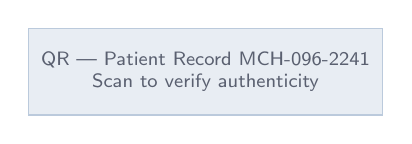
\begin{tikzpicture}
      \fill[PedBlue!10] (0,0) rectangle (4.5cm, 1.1cm);
      \draw[PedBlue!30, line width=0.5pt] (0,0) rectangle (4.5cm, 1.1cm);
      \node[font=\fontsize{7}{8}\selectfont, text=GrayText, align=center]
        at (2.25cm, 0.55cm) {QR --- Patient Record MCH-096-2241\\
        Scan to verify authenticity};
    \end{tikzpicture}
  \end{minipage}
\end{tcolorbox}

\vspace{3mm}

%% ── Footer rule ─────────────────────────────────────────────────────────────
{\color{PedTeal}\rule{\linewidth}{0.4pt}}\\[-3pt]
{\color{PedBlue}\rule{\linewidth}{1.5pt}}

\vspace{1mm}
{\footnotesize\color{GrayText}\centering
\textbf{Meridian Children's Hospital} \textbar\
47 Lakeview Blvd, Suite 300, Harborfield ON M4K 2R7 \textbar\
Tel: (416) 555-0182 \textbar\ Fax: (416) 555-0199\\
\textbf{CONFIDENTIAL --- This document contains privileged patient health information.
Unauthorized disclosure is prohibited under applicable privacy legislation.}\\
\textit{This document is a SPECIMEN for template demonstration purposes only.
All patient, provider, and institutional details are entirely fictional.}
}

\end{document}
